%%%%%%%%%%%%%%%%%%%
\section[Building Blocks]{2. Building Blocks of Deep Architectures}
\begin{frame}
\small{\frametitle{Outline}
\tableofcontents
}
\end{frame}
%%%%%%%%%%%%%%%%%%%%


%% SUBSECTION%%%%%
\subsection[RBM]{Restricted Boltzmann Machines (RBM)}

%%%%%%%%%%%%%%%%
\begin{frame}
\frametitle{Deep Learning Paradigm}
\bi
\item Recall problem setup: Learn function {\color{red} $f: x \rightarrow y$ }
\pause
\item First learn hidden features $h$ that model input, i.e.  {\color{red} $x \rightarrow h \rightarrow y$}
\pause
\item How to discover useful latent features $h$ from data $x$? 
\bi 
	\item We'll focus on unsupervised techniques, e.g. use Restricted Boltzmann Machines (RBMs)
\ei
\ei
\end{frame}




%%%%%%%
\begin{frame}
\frametitle{Restricted Boltzmann Machine (RBM)}
\bi
\item RBM is a probabilistic model on binary variables $h_j$, $x_i$:\\
\begin{eqnarray*} 
p(x,h) &=& \frac{1}{Z_\theta} \exp{( - E_\theta(x,h))}\\
         &=& \frac{1}{Z_\theta} \exp{( x^T W h + b^T x + d^T h )}
\end{eqnarray*}
	\bi
	\item $W$ is a matrix; elements $W_{ij}$ models correlation between $x_i$ and $h_j$
	\item $b$ and $d$ are bias terms; we'll assume $b=d=0$ here.
	\item normalizer (partition function): $Z_\theta = \sum_{(x,h)} \exp(-E_\theta(x,h))$ 
	\ei
	\begin{center}
\begin{tikzpicture}[-,>=stealth',shorten >=1pt,auto,node distance=3cm,
  thick,main node/.style={circle,fill=blue!20,draw,font=\sffamily\Large\bfseries}]

  \node[main node] (x1) at (0,0) {$x_1$};
  \node[main node] (x2) at (2,0) {$x_2$};
  \node[main node] (x3) at (4,0) {$x_3$};
  \node[main node] (h1) at (0,2) {$h_1$};
  \node[main node] (h2) at (2,2) {$h_2$};
  \node[main node] (h3) at (4,2) {$h_3$};

  \path[every node/.style={font=\sffamily\small}]
    (x1) edge node [left] {$W_{ij}$} (h1)
    (x1) edge node {} (h2)
    (x1) edge node {} (h3)
    (x2) edge node {} (h1)
    (x2) edge node {} (h2)
    (x2) edge node {} (h3)
    (x3) edge node {} (h1)
    (x3) edge node {} (h2)
    (x3) edge node {} (h3);
\end{tikzpicture}
\end{center}
\ei
\end{frame}


%%%%%%%
\begin{frame}
\frametitle{Restricted Boltzmann Machine (RBM): Example}
\begin{center}
\begin{tikzpicture}[-,>=stealth',shorten >=1pt,auto,node distance=3cm,
  thick,main node/.style={circle,fill=blue!20,draw,font=\sffamily\Large\bfseries}]

  \node[main node] (x1) at (0,0) {$x_1$};
  \node[main node] (x2) at (2,0) {$x_2$};
  \node[main node] (x3) at (4,0) {$x_3$};
  \node[main node] (h1) at (0,2) {$h_1$};
  \node[main node] (h2) at (2,2) {$h_2$};
  \node[main node] (h3) at (4,2) {$h_3$};

  \path[every node/.style={font=\sffamily\small}]
    (x1) edge node {} (h2)
    (x2) edge node {} (h1)
    (x2) edge node {} (h2)
    (x2) edge node {} (h3)
    (x3) edge node {} (h1)
    (x3) edge node {} (h2)
    (x3) edge node {} (h3);

  \path[red, very thick, every node/.style={font=\sffamily\small}]
    (x1) edge node {} (h1)
    (x1) edge node {} (h3);
\end{tikzpicture}

Let $W_{ij}$ on edges $(h_1,x_1), (h_3,x_1)$ be big positive, others be small negative. 

\begin{tabular}{|c|c|c|c|c|c||c|}
\hline
$x_1$ & $x_2$ & $x_3$  & $h_1$ & $h_2$ & $h_3$ & $p(x,h)= \frac{1}{Z_\theta} \exp{( x^T W h  )}$ \\\hline\hline
   1      &	  0    &    0       &    1     &     0     &     1     & highest \\ \hline
   1      &	  0    &    0       &    0     &     0     &     1     & high \\ \hline
   1      &	  0    &    0       &    1     &     0     &     0     & high \\ \hline
   0      &	  0    &    0       &    1     &     0     &     1     & low \\ \hline
   0      &	  1    &    0       &    0     &     0     &     0     & low \\ \hline
   0      &	  0    &    1       &    0     &     0     &     0     & low \\ \hline
\end{tabular}

etc
\end{center}
\end{frame}


\begin{frame}[plain]
\frametitle{RBM Posterior Distribution (Easy!)}
\bi
\item Computing $p(h|x)$ is easy due to factorization:
\begin{eqnarray*} 
\hspace{-1cm}{\color{red} p(h|x)} & = &  \frac{p(x,h)}{\sum_h p(x,h)} = \frac{1/Z_\theta \exp(-\Es)}{\sum_h 1/Z_\theta \exp(-\Es)}\\
	 & = & \frac{\exp(x^T W h + b^T x + d^T h)}{\sum_h \exp(x^T W h + b^T x + d^T h)}\\
	& = &  \frac{\prod_j \exp(x^T W_j h_j +  d_j h_j)\cdot \exp(b^Tx)}{\sum_{h_1\in\{0,1\}} \sum_{h_2\in\{0,1\}}\cdots \sum_{h_j} \prod_j\exp(x^T W_j h_j +  d_j h_j)\cdot \exp(b^Tx)}\\
	& = &  \frac{  \prod_j \exp(x^T W_j h_j +  d_j h_j)}{\prod_j \sum_{h_j\in\{0,1\}}   \exp(x^T W_j h_j +  d_j h_j)}\\\
	& = & \prod_j \frac{\exp(x^T W_j h_j +  d_j h_j)}{\sum_{h_j\in\{0,1\}}   \exp(x^T W_j h_j +  d_j h_j)} = {\color{red} \prod_j p(h_j|x)}\\
\end{eqnarray*}
\item ${\color{red} p(h_j=1|x) = \exp(x^T W_j +  d_j)/Z = \sigma(x^T W_j +  d_j)}$ \small{is Logistic Regression!}
\pause
\item Similarly, computing $p(x|h)=\prod_i p(x_i|h)$ is easy
\ei
\end{frame}


%%%%%%%%%%%%%
\begin{frame}[plain]
\frametitle{RBM Max-Likelihood Training (Hard!)}
Derivative of the Log-Likelihood: ${\color{red} \nw \log P_w(x=x^{(m)})}$
\begin{small}
\begin{eqnarray}
&=& \nw \log \sum_{h} P_w(x=x^{(m)},h) \\
&=& \nw \log \sum_h \frac{1}{Z_w} \exp{(-\Em)}\\
&=& -\nw \log Z_w + \nw \log \sum_h \exp{(-\Em)}  \\
& & \hspace{-12mm} =\frac{1}{Z_w} \sum_{h,x} e^{(-\E)} \nw \E - \frac{1}{\sum_h e^{(-\Em)}} \sum_h e^{(-\Em)} \nw \Em  \nonumber \\ 
&=& \sum_{h,x} P_w(x,h) [\nw \E] - \sum_h P_w(x^{(m)},h) [\nw \Em] \\
&=& {\color{red} - \mathbb{E}_{p(x,h)} [ x_i \cdot h_j ] + \mathbb{E}_{p(h|x=x^{(m)})} [ x^{(m)}_i \cdot h_j ]}
\end{eqnarray}
\end{small}
\pause
Second term (positive phase) increases probability of $x^{(m)}$; First term (negative phase) decreases probability of samples generated by the model
\end{frame}

%%%%%%%%%%%%%
\begin{frame}
\frametitle{Contrastive Divergence Algorithm}
\begin{center}
\scalebox{0.7}{
\begin{tikzpicture}[-,>=stealth',shorten >=1pt,auto,node distance=3cm,
  thick,main node/.style={circle,fill=blue!20,draw,font=\sffamily\Large\bfseries}]

  \node[main node] (x1) at (0,0) {$x_1$};
  \node[main node] (x2) at (2,0) {$x_2$};
  \node[main node] (x3) at (4,0) {$x_3$};
  \node[main node] (h1) at (0,2) {$h_1$};
  \node[main node] (h2) at (2,2) {$h_2$};
  \node[main node] (h3) at (4,2) {$h_3$};

  \path[every node/.style={font=\sffamily\small}]
    (x1) edge node {} (h1)
    (x1) edge node {} (h2)
    (x1) edge node {} (h3)
    (x2) edge node {} (h1)
    (x2) edge node {} (h2)
    (x2) edge node {} (h3)
    (x3) edge node {} (h1)
    (x3) edge node {} (h2)
    (x3) edge node {} (h3);
\end{tikzpicture}
}
\end{center}
\bi
\item The negative phase term ($\mathbb{E}_{p(x,h)} [ x_i \cdot h_j ]$) is expensive because it requires sampling (x,h) from the model
\pause
\item Gibbs Sampling works but slow.
\pause
\item Contrastive Divergence (faster but biased):
\pause
	\be
	\item Let $x^{(m)}$ be training point,\\$W=[w_{ij}]$ be current model weights 
	\item Sample $\hat{h}_j \in \{0,1\}$ from $p(h_j|x=x^{(m)})=\sigma(\sum_i w_{ij}x^{(m)}_i + d_j )$
	\item Sample $\tilde{x}_i \in \{0,1\}$ from $p(x_i|h=\hat{h})=\sigma(\sum_j w_{ij}\hat{h}_j + b_i )$
	\item Sample $\tilde{h}_j \in \{0,1\}$ from $p(h_j|x=\tilde{x})=\sigma(\sum_i w_{ij}\tilde{x}_i + d_j )$
	\item $w_{ij} \leftarrow w_{ij} + \gamma( x^{(m)}_i \cdot \hat{h}_j - \tilde{x}_i \cdot \tilde{h}_j) $
	\ee
\ei
\end{frame}

%%%%%%%%%%%%%
\begin{frame}
\frametitle{Contrastive Divergence Pictorial View}
\bi
\item Goal: Make RBM $p(x,h)$ have high probability on training samples
\item To do so, we'll "steal" probability mass from nearby samples that incorrectly preferred by the model
\item Analysis in \cite{carreira05cd}  
\ei
\centerline{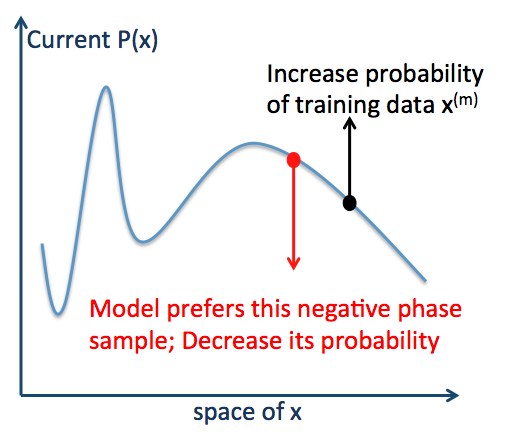
\includegraphics[scale=0.4]{figs/contrastive_divergence}}
\end{frame}


%%%%%%%%
\begin{frame}
\frametitle{Distributed Representations learned by RBM}
\bi
\item Vector $h$ act as \textbf{Distributed Representation} of data 
	\bi
	\item Multiple $h_j$ may be active simultaneously for a given $x$. (Multi-clustering)
	\item $2^{|h|}$ possible representations with $|h|\times|x|$ parameters. 
	\ei
\begin{center}
\scalebox{0.8}{
\begin{tikzpicture}[-,>=stealth',shorten >=1pt,auto,node distance=3cm,
  thick,main node/.style={circle,fill=blue!20,draw,font=\sffamily\Large\bfseries}]

  \node[main node] (x1) at (0,0) {$x_1$};
  \node[main node] (x2) at (2,0) {$x_2$};
  \node[main node] (x3) at (4,0) {$x_3$};
  \node[main node] (h1) at (0,2) {$h_1$};
  \node[main node] (h2) at (2,2) {$h_2$};
  \node[main node] (h3) at (4,2) {$h_3$};

  \path[every node/.style={font=\sffamily\small}]
    (x1) edge node {} (h1)
    (x1) edge node {} (h2)
    (x1) edge node {} (h3)
    (x2) edge node {} (h1)
    (x2) edge node {} (h2)
    (x2) edge node {} (h3)
    (x3) edge node {} (h1)
    (x3) edge node {} (h2)
    (x3) edge node {} (h3);
\end{tikzpicture}
}
\end{center}

\pause
\item A mixture model $p(x)=\sum_h p(c)p(x|c)$ would need $2^{|h|} \times |x|$ parameters:

\begin{center}
\scalebox{0.8}{
\begin{tikzpicture}[<-,>=stealth',shorten >=1pt,auto,node distance=3cm,
  thick,main node/.style={circle,fill=blue!20,draw,font=\sffamily\Large\bfseries}]

  \node[main node] (x1) at (0,0) {$x_1$};
  \node[main node] (x2) at (2,0) {$x_2$};
  \node[main node] (x3) at (4,0) {$x_3$};
  \node[main node] (h1) at (2,2) {$c$};
  

  \path[every node/.style={font=\sffamily\small}]
    (x1) edge node {} (h1)
    (x2) edge node {} (h1)
    (x3) edge node {} (h1);
\end{tikzpicture}
}
\end{center}


\ei
\end{frame}

%%%%%
\begin{frame}
\frametitle{Layer-wise Pre-training of RBMs}
\begin{columns}
\begin{column}{0.5\textwidth}
\begin{center}
\scalebox{0.8}{
\begin{tikzpicture}[-,>=stealth',shorten >=1pt,auto,node distance=3cm,
  thick,main node/.style={circle,fill=blue!20,draw,font=\sffamily\Large\bfseries}]

  \node[main node] (x1) at (0,0) {$x_1$};
  \node[main node] (x2) at (2,0) {$x_2$};
  \node[main node] (x3) at (4,0) {$x_3$};
  \node[main node] (h1) at (0,2) {$h_1$};
  \node[main node] (h2) at (2,2) {$h_2$};
  \node[main node] (h3) at (4,2) {$h_3$};
  \node[main node] (h'1) at (0,4) {$h'_1$};
  \node[main node] (h'2) at (2,4) {$h'_2$};
  \node[main node] (h'3) at (4,4) {$h'_3$};
  \node[main node] (h''1) at (0,6) {$h''_1$};
  \node[main node] (h''2) at (2,6) {$h''_2$};
  \node[main node] (h''3) at (4,6) {$h''_3$};
  \node at (5.1,1) {Layer1 RBM};
  \node at (5.1,3) {Layer2 RBM};
  \node at (5.1,5) {Layer3 RBM};

    \path[every node/.style={font=\sffamily\small}]
    (x1) edge node {} (h1)
    (x1) edge node {} (h2)
    (x1) edge node {} (h3) 
    (x2) edge node {} (h1)
    (x2) edge node {} (h2)
    (x2) edge node {} (h3) 
    (x3) edge node {} (h1)
    (x3) edge node {} (h2)
    (x3) edge node {} (h3)
    (h1) edge node {} (h'1)
    (h1) edge node {} (h'2)
    (h1) edge node {} (h'3)
    (h2) edge node {} (h'1)
    (h2) edge node {} (h'2)
    (h2) edge node {} (h'3)
    (h3) edge node {} (h'1)
    (h3) edge node {} (h'2)
    (h3) edge node {} (h'3)
    (h'1) edge node {} (h''1)
    (h'1) edge node {} (h''2)
    (h'1) edge node {} (h''3)
    (h'2) edge node {} (h''1)
    (h'2) edge node {} (h''2)
    (h'2) edge node {} (h''3)
    (h'3) edge node {} (h''1)
    (h'3) edge node {} (h''2)
    (h'3) edge node {} (h''3)
    ;

\end{tikzpicture}
}
\end{center}
\end{column}
\begin{column}{0.4\textwidth}
\be
\item Train Layer 1 RBM\\max $\log P(x,h)$
\item Train Layer 2 RBM\\max $\log P(h,h')$
\item Train Layer 3 RBM\\max $\log P(h',h'')$
\ee
\end{column}
\end{columns}
\end{frame}

%%%%%
\begin{frame}
\frametitle{Deep Belief Nets (DBN) =  Stacked RBM \cite{hinton06dbn}}
\begin{columns}
\begin{column}{0.4\textwidth}
\begin{center}
\scalebox{0.8}{
\begin{tikzpicture}[-,>=stealth',shorten >=1pt,auto,node distance=3cm,
  thick,main node/.style={circle,fill=blue!20,draw,font=\sffamily\Large\bfseries}]

  \node[main node] (x1) at (0,0) {$x_1$};
  \node[main node] (x2) at (2,0) {$x_2$};
  \node[main node] (x3) at (4,0) {$x_3$};
  \node[main node] (h1) at (0,2) {$h_1$};
  \node[main node] (h2) at (2,2) {$h_2$};
  \node[main node] (h3) at (4,2) {$h_3$};
  \node[main node] (h'1) at (0,4) {$h'_1$};
  \node[main node] (h'2) at (2,4) {$h'_2$};
  \node[main node] (h'3) at (4,4) {$h'_3$};
  \node[main node] (h''1) at (0,6) {$h''_1$};
  \node[main node] (h''2) at (2,6) {$h''_2$};
  \node[main node] (h''3) at (4,6) {$h''_3$};
  \node at (4.6,1) {Layer1};
  \node at (4.6,3) {Layer2};
  \node at (4.6,5) {Layer3};


  \path[<-,every node/.style={font=\sffamily\small}]
    (x1) edge node {} (h1)
    (x1) edge node {} (h2)
    (x1) edge node {} (h3) 
    (x2) edge node {} (h1)
    (x2) edge node {} (h2)
    (x2) edge node {} (h3) 
    (x3) edge node {} (h1)
    (x3) edge node {} (h2)
    (x3) edge node {} (h3)
    (h1) edge node {} (h'1)
    (h1) edge node {} (h'2)
    (h1) edge node {} (h'3)
    (h2) edge node {} (h'1)
    (h2) edge node {} (h'2)
    (h2) edge node {} (h'3)
    (h3) edge node {} (h'1)
    (h3) edge node {} (h'2)
    (h3) edge node {} (h'3);
    
    \path[every node/.style={font=\sffamily\small}]
    (h'1) edge node {} (h''1)
    (h'1) edge node {} (h''2)
    (h'1) edge node {} (h''3)
    (h'2) edge node {} (h''1)
    (h'2) edge node {} (h''2)
    (h'2) edge node {} (h''3)
    (h'3) edge node {} (h''1)
    (h'3) edge node {} (h''2)
    (h'3) edge node {} (h''3)
    ;

\end{tikzpicture}
}
\end{center}
\end{column}
\begin{column}{0.6\textwidth}
\bi
\item After pre-training, stacked RBM can be converted to DBN, defined as: $p(x)=\sum_{h,h',h''}p(x|h)p(h|h')p(h',h'')$\pause
\item This is a probabilistic generative model: Can sample from RBM at Layer3, then generate data $x$ via directed sigmoids \pause
\item Upper layers can be viewed as prior; More layers = better prior
\ei
\end{column}
\end{columns}
\end{frame}


%%%%%
\begin{frame}
\frametitle{Popular alternative: Initialize MLP with RBMs}
\begin{columns}
\begin{column}{0.4\textwidth}
\begin{center}
\scalebox{0.8}{
\begin{tikzpicture}[-,>=stealth',shorten >=1pt,auto,node distance=3cm,
  thick,main node/.style={circle,fill=blue!20,draw,font=\sffamily\Large\bfseries}]

  \node[main node] (x1) at (0,0) {$x_1$};
  \node[main node] (x2) at (2,0) {$x_2$};
  \node[main node] (x3) at (4,0) {$x_3$};
  \node[main node] (h1) at (0,2) {$h_1$};
  \node[main node] (h2) at (2,2) {$h_2$};
  \node[main node] (h3) at (4,2) {$h_3$};
  \node[main node] (h'1) at (0,4) {$h'_1$};
  \node[main node] (h'2) at (2,4) {$h'_2$};
  \node[main node] (h'3) at (4,4) {$h'_3$};
  \node[main node] (h''1) at (0,6) {$h''_1$};
  \node[main node] (h''2) at (2,6) {$h''_2$};
  \node[main node] (h''3) at (4,6) {$h''_3$};
  \node at (4.6,1) {Layer1};
  \node at (4.6,3) {Layer2};
  \node at (4.6,5) {Layer3};
  \node[main node] (y) at (2,8) {$y$};

  \path[->,every node/.style={font=\sffamily\small}]
    (x1) edge node {} (h1)
    (x1) edge node {} (h2)
    (x1) edge node {} (h3) 
    (x2) edge node {} (h1)
    (x2) edge node {} (h2)
    (x2) edge node {} (h3) 
    (x3) edge node {} (h1)
    (x3) edge node {} (h2)
    (x3) edge node {} (h3)
    (h1) edge node {} (h'1)
    (h1) edge node {} (h'2)
    (h1) edge node {} (h'3)
    (h2) edge node {} (h'1)
    (h2) edge node {} (h'2)
    (h2) edge node {} (h'3)
    (h3) edge node {} (h'1)
    (h3) edge node {} (h'2)
    (h3) edge node {} (h'3);
    
    \path[->,every node/.style={font=\sffamily\small}]
    (h'1) edge node {} (h''1)
    (h'1) edge node {} (h''2)
    (h'1) edge node {} (h''3)
    (h'2) edge node {} (h''1)
    (h'2) edge node {} (h''2)
    (h'2) edge node {} (h''3)
    (h'3) edge node {} (h''1)
    (h'3) edge node {} (h''2)
    (h'3) edge node {} (h''3)
    ;

    \path[->,every node/.style={font=\sffamily\small}]
    (h''1) edge node {} (y)
    (h''2) edge node {} (y)
    (h''3) edge node {} (y)
    ;

\end{tikzpicture}
}
\end{center}
\end{column}
\begin{column}{0.6\textwidth}
\bi
\item {Stacked RBMs can be used to initialize a Deep Neural Network (DNN), i.e. MLP}
\item {Then, fine-tuned by back-propagation}
\ei
\end{column}
\end{columns}
\end{frame}



%%%%%%%%%%%%%
\begin{frame}
\frametitle{What a Deep Generative Model can do}
After training on 20k images, the generative model of \cite{salakhutdinov09dbm}* can generate random images (dimension=8976) that are amazingly realistic!
\vspace{1cm} 
\centerline{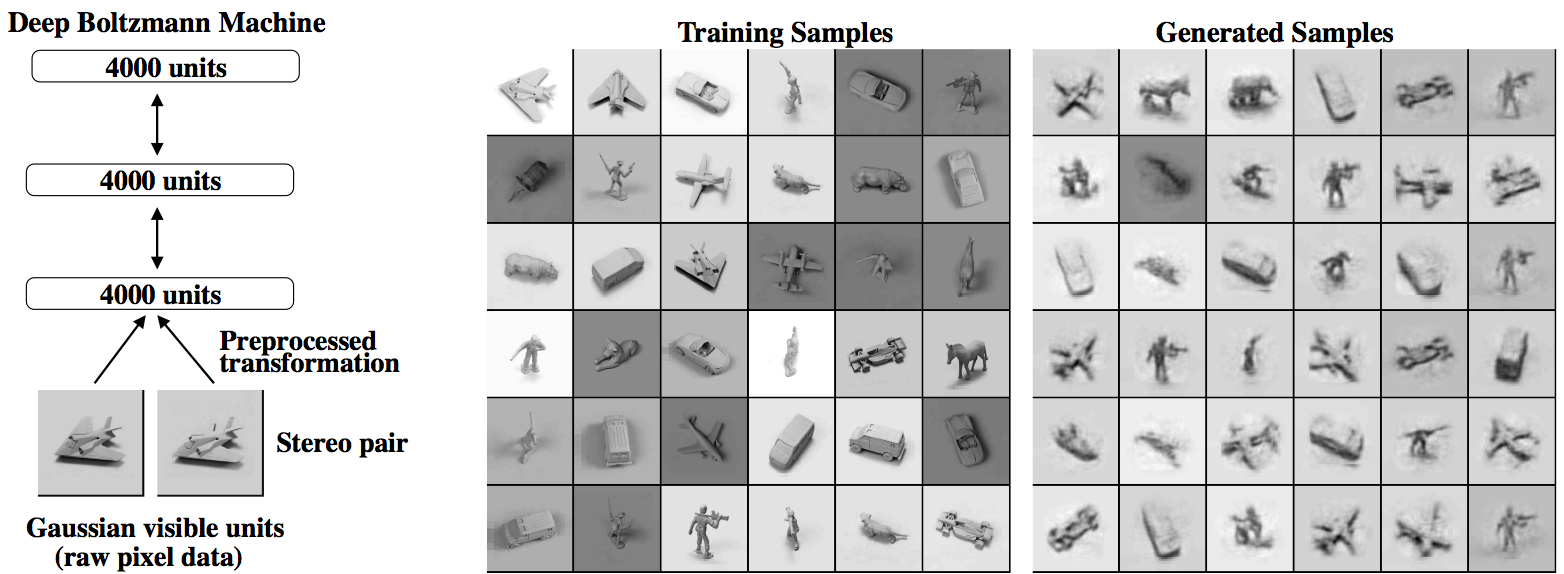
\includegraphics[scale=0.17]{figs/dbm_generation}}
\blfootnote{This model is a Deep Boltzmann Machine (DBM), different from Deep Belief Nets (DBN) but also built by stacking RBMs.}
\end{frame}

%%%%%%%%%%%%%
\begin{frame}
\frametitle{RBM and DBN Summary}
\be
\item Layer-wise pre-training is the innovation that rekindled interest in deep architectures. \pause
\item Pre-training focuses on optimizing likelihood on the data, not label. First model $p(x)$ to do better $p(y|x)$. \pause
\item Why RBM? $p(h|x)$ is tractable, so it's easy to stack.\pause
\item RBM training can be expensive. Solution: contrastive divergence\pause
\item We can stack RBMs to form a deep probabilistic generative model (DBN), or to initialize deep neural network (DNN) 
\ee
\end{frame}


%%%%%%%%%
\subsection[Auto-Encoders]{Auto-Encoders}

\begin{frame}
\frametitle{Auto-Encoders: Efficient replacement for RBM}

\begin{center}
\begin{tikzpicture}[->,>=stealth',shorten >=1pt,auto,node distance=3cm,
  thick,main node/.style={circle,fill=blue!20,draw,font=\sffamily\Large\bfseries}]

  \node[main node] (x1) at (0,0) {$x_1$};
  \node[main node] (x2) at (2,0) {$x_2$};
  \node[main node] (x3) at (4,0) {$x_3$};
  \node[main node] (h1) at (1,2) {$h_1$};
  \node[main node] (h2) at (3,2) {$h_2$};
  \node[main node] (h'1) at (0,4) {$x'_1$};
  \node[main node] (h'2) at (2,4) {$x'_2$};
  \node[main node] (h'3) at (4,4) {$x'_3$};
  \node at (7,1) {Encoder: $h =\sigma(Wx+b)$ };
  \node at (7,3) {Decoder: $x' =\sigma(W'h+d)$};


  \path[every node/.style={font=\sffamily\small}]
    (x1) edge node {} (h1)
    (x1) edge node {} (h2)
    (x2) edge node {} (h1)
    (x2) edge node {} (h2)
    (x3) edge node {} (h1)
    (x3) edge node {} (h2)
    (h1) edge node {} (h'1)
    (h1) edge node {} (h'2)
    (h1) edge node {} (h'3)
    (h2) edge node {} (h'1)
    (h2) edge node {} (h'2)
    (h2) edge node {} (h'3);

\end{tikzpicture}
\end{center}
\pause
Encourage $h$ to give small reconstruction error:
	\bi
	\item $Loss = \sum_m || x^{(m)} - DECODER(ENCODER(x^{(m)})) ||^2 $\pause
	\item Reconstruction: $x' =\sigma(W'\sigma(Wx+b)+d)$\pause
	\item $|h|$ is small to enforce "compression" of data \pause
	\item Back-prop for 2-layer nets, with $x^{(m)}$ as input \& output
	\ei
\end{frame}



%%%%%%%%%
\begin{frame}
\frametitle{Stacked Auto-Encoders (SAE) \cite{bengio06greedy}}
\bi 
\item The encoder/decoder gives same form $p(h|x)$, $p(x|h)$ as RBMs, so can be stacked in the same way
\pause
\begin{center}
\scalebox{0.65}{\begin{tikzpicture}[->,>=stealth',shorten >=1pt,auto,node distance=3cm,
  thick,main node/.style={circle,fill=blue!20,draw,font=\sffamily\Large\bfseries}]

  \node[main node] (x1) at (0,0) {$x_1$};
  \node[main node] (x2) at (2,0) {$x_2$};
  \node[main node] (x3) at (4,0) {$x_3$};
  \node[main node] (x4) at (6,0) {$x_4$};
  \node[main node] (h1) at (1,2) {$h_1$};
  \node[main node] (h2) at (3,2) {$h_2$};
  \node[main node] (h3) at (5,2) {$h_3$};
  \node[main node] (h'1) at (2,4) {$h'_1$};
  \node[main node] (h'2) at (4,4) {$h'_2$};
  \node[main node] (y) at (3,6) {$y$};
  \node at (7,1) {Layer1 Encoder};
  \node at (7,3) {Layer2 Encoder};
  \node at (7,5) {Output layer};


  \path[every node/.style={font=\sffamily\small}]
    (x1) edge node {} (h1)
    (x1) edge node {} (h2)
    (x1) edge node {} (h3)
    (x2) edge node {} (h1)
    (x2) edge node {} (h2)
    (x2) edge node {} (h3)
    (x3) edge node {} (h1)
    (x3) edge node {} (h2)
    (x3) edge node {} (h3)
    (x4) edge node {} (h1)
    (x4) edge node {} (h2)
    (x4) edge node {} (h3)
    (h1) edge node {} (h'1)
    (h1) edge node {} (h'2)
    (h2) edge node {} (h'1)
    (h2) edge node {} (h'2)
    (h3) edge node {} (h'1)
    (h3) edge node {} (h'2)
    (h'1) edge node {} (y)
    (h'2) edge node {} (y)
  
    ;
\end{tikzpicture}}
\end{center}

\pause
\item Unlike RBMs, Auto-encoders are deterministic. 
	\bi
	\item $h =\sigma(Wx+b)$, not $p(h=1) =\sigma(Wx+b)$\pause
	\item Disadvantage: Can't form deep generative model
	\item Advantage: Fast to train, useful still for DNN init
	\ei
\item Note similarities to RBM contrastive divergence 
\ei

\end{frame}


\begin{frame}
\frametitle{Variants: e.g. Denoising Auto-Encoder}

\begin{center}
\begin{tikzpicture}[->,>=stealth',shorten >=1pt,auto,node distance=3cm,
  thick,main node/.style={circle,fill=blue!20,draw,font=\sffamily\Large\bfseries}]

  \node[main node] (x1) at (0,0) {$\tilde{x_1}$};
  \node[main node] (x2) at (2,0) {$\tilde{x_2}$};
  \node[main node] (x3) at (4,0) {$\tilde{x_3}$};
  \node[main node] (h1) at (1,2) {$h_1$};
  \node[main node] (h2) at (3,2) {$h_2$};
  \node[main node] (h'1) at (0,4) {$x'_1$};
  \node[main node] (h'2) at (2,4) {$x'_2$};
  \node[main node] (h'3) at (4,4) {$x'_3$};
  \node at (7,0) {$\tilde{x} = x + $ noise};
  \node at (7,1) {Encoder: $h =\sigma(W\tilde{x}+b)$ };
  \node at (7,3) {Decoder: $x' =\sigma(W'h+d)$};


  \path[every node/.style={font=\sffamily\small}]
    (x1) edge node {} (h1)
    (x1) edge node {} (h2)
    (x2) edge node {} (h1)
    (x2) edge node {} (h2)
    (x3) edge node {} (h1)
    (x3) edge node {} (h2)
    (h1) edge node {} (h'1)
    (h1) edge node {} (h'2)
    (h1) edge node {} (h'3)
    (h2) edge node {} (h'1)
    (h2) edge node {} (h'2)
    (h2) edge node {} (h'3)
    ;

\end{tikzpicture}
\end{center}

\be
\item Perturb input data $x$ to $\tilde{x}$ using invariance from domain knowledge. 
\item Train weights to reduce reconstruction error with respect to original input: $||x-x'||$
\ee
\end{frame}


\begin{frame}
\frametitle{Denoising Auto-Encoders}
\bi
\item Example: Randomly shift, rotate, and scale input image
\item An image of "2" is a "2" no matter how you add noise, so the auto-encoder will try to cancel the variations that are not important. 
\ei
\centerline{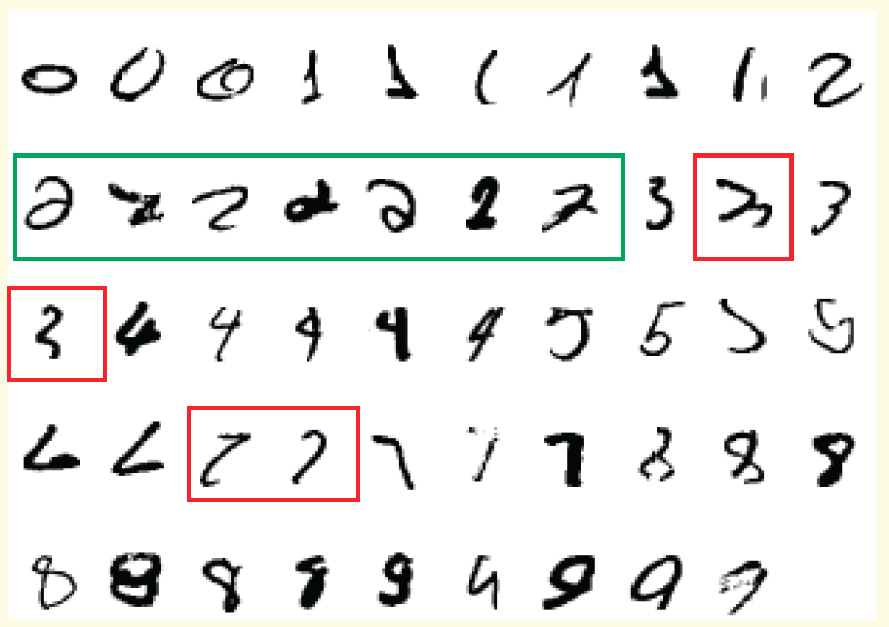
\includegraphics[scale=0.19]{figs/digit2}}
\blfootnote{Figure from Geoff Hinton's 2012 Coursera course, lecture 1: \url{https://www.coursera.org/course/neuralnets}}
\end{frame}

%%%%%%%%%%%%%%%%%%%%%%%%%%%%%%%%%%%%%%
\begin{frame}
\frametitle{Stacked Auto-Encoders (SAE): Summary}
\be
\item Auto-Encoders are cheaper alternatives to RBMs.
	\bi
	\item Not probabilistic, but fast to train using Backpropagation
	\item Achieves similar accuracies as RBM \cite{bengio06greedy}
	\ei
\pause
\item Auto-Encoders learn to "compress" and "re-construct" input data. Again, the focus is on modeling $p(x)$ first.  \pause
\item Many variants, some provide ways to incorporate domain knowledge.
\ee
\end{frame}


%%%%%%%%%
\subsection[Recurrent Units]{Recurrent Units}

\begin{frame}
\frametitle{Modeling sequence data}
\centerline{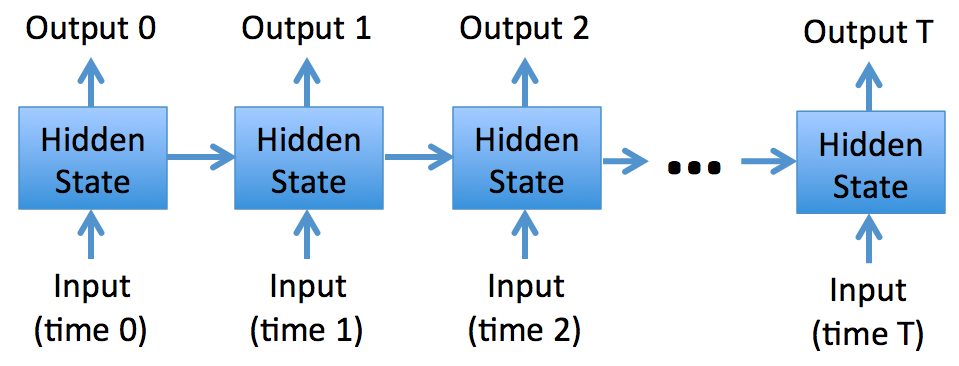
\includegraphics[scale=0.3]{figs/sequencemodel}}
\bi
\pause
\item Example applications:
  
	\bi 
        \item Time-series prediction
        \item Sequence-to-sequence transduction
	\item Language modeling $P(current\_word \mid previous\_words)$
	\ei
\ei
\end{frame}


\begin{frame}
\frametitle{Recurrent Neural Net Language Models}
Model $p(current\_word|previous\_words)$ with a recurrent hidden layer \cite{mikolov10rnnlm}

\begin{columns}
\column{0.6\textwidth}
\scalebox{0.6}{\begin{tikzpicture}[->,>=stealth',shorten >=1pt,auto,node distance=3cm,
  thick,main node/.style={circle,fill=blue!20,draw,font=\sffamily\Large\bfseries}]

  \node[main node] (x1) at (0,0) {$x_1$};
  \node[main node] (x2) at (2,0) {$x_2$};
  \node[main node] (x3) at (4,0) {$x_3$};
  \node[main node] (x4) at (6,0) {$x_4$};
  \node[main node] (x5) at (8,0) {$x_5$};
  \node[main node] (h1) at (4,2) {$h_1$};
  \node[main node] (h2) at (6,2) {$h_2$};
  \node[main node] (h'1) at (0,4) {$y_1$};
  \node[main node] (h'2) at (2,4) {$y_2$};
  \node[main node] (h'3) at (4,4) {$y_3$};

  \draw[blue,ultra thick,-latex,<->] (0,-1) -- node[]{Previous Word} (4,-1);
  \draw[blue,ultra thick,-latex,<->] (6,-1) -- node[]{Previous $h$} (8,-1);
  \draw[blue,ultra thick,-latex,<->] (0,5) -- node[]{Current Word (assume 3-word vocabulary)} (4,5);

   \node(wij) at (1,1) {$w_{ij}$};
   \node(wjk) at (1,3) {$w_{jk}$};

  \path[every node/.style={font=\sffamily\small}]
    (x1) edge node {} (h1)
    (x2) edge node {} (h1)
    (x3) edge node {} (h1)
    (x4) edge node {} (h1)
    (x5) edge node {} (h1)
    (x1) edge node {} (h2)
    (x2) edge node {} (h2)
    (x3) edge node {} (h2)
    (x4) edge node {} (h2)
    (x5) edge node {} (h2)
    (h1) edge node {} (h'1)
    (h2) edge node {} (h'1)
    (h1) edge node {} (h'2)
    (h2) edge node {} (h'2)
    (h1) edge node {} (h'3)
    (h2) edge node {} (h'3)
    ;
\end{tikzpicture}}
    \column{.4\textwidth}
\bi
\item Probability of word: $y_k=\frac{\exp(W_{jk}^T h)}{\sum_{k'}\exp(W_{jk'}^T h)}$
\item $[x_4,x_5]$ is a copy of $[h_1,h_2]$ from the previous time-step
\item $h_j=\sigma(W_{ij}^T x_i)$ is hidden state of partial sentence
\item Arbitrarily-long history is (theoretically) kept through recurrence
\ei
\end{columns}
\end{frame}

\begin{frame}
\frametitle{Training: Backpropagation through Time}
Unroll the hidden states for a few time-steps, then backprop.\\
{\color{red} Very deep network: vanishing/exploding gradients!}

\scalebox{0.8}{\begin{tikzpicture}[->,>=stealth',shorten >=1pt,auto,node distance=3cm,
  thick,main node/.style={circle,fill=blue!20,draw,font=\sffamily\Large\bfseries}]

  \node[main node] (x1) at (0,0) {$x_1$};
  \node[main node] (x2) at (2,0) {$x_2$};
  \node[main node] (x3) at (4,0) {$x_3$};
  \node[main node] (x4) at (6,0) {$h'_1$};
  \node[main node] (x5) at (8,0) {$h'_2$};
  \node[main node] (h1) at (4,2) {$h_1$};
  \node[main node] (h2) at (6,2) {$h_2$};
  \node[main node] (h'1) at (0,4) {$y_1$};
  \node[main node] (h'2) at (2,4) {$y_2$};
  \node[main node] (h'3) at (4,4) {$y_3$};

  \node[main node] (px1) at (2,-3) {$x_1$};
  \node[main node] (px2) at (4,-3) {$x_2$};
  \node[main node] (px3) at (6,-3) {$x_3$};
  \node[main node] (px4) at (8,-3) {$h''_1$};
  \node[main node] (px5) at (10,-3) {$h''_2$};

  \draw[blue,ultra thick,-latex,<->] (2,-4) -- node[]{"Input0" $[x_1,x_2,x_3]=[0,1,0]$} (6,-4);
  \draw[blue,ultra thick,-latex,<->] (0,-1) -- node[]{"Input1" $[x_1,x_2,x_3]=[1,0,0]$} (4,-1);
 \draw[blue,ultra thick,-latex,<->] (6,-1) -- node[]{Previous $h$} (8,-1);
\draw[blue,ultra thick,-latex,<->] (8,-4) -- node[]{Initial $h$} (10,-4);
   \node(wij) at (1,1) {$w_{ij}$};
   \node(wjk) at (1,3) {$w_{jk}$};
      \node(wij) at (3,-2) {$w_{ij}$};

  \path[every node/.style={font=\sffamily\small}]
    (px1) edge node {} (x4)
    (px2) edge node {} (x4)
    (px3) edge node {} (x4)
    (px4) edge node {} (x4)
    (px5) edge node {} (x4)
    (px1) edge node {} (x5)
    (px2) edge node {} (x5)
    (px3) edge node {} (x5)
    (px4) edge node {} (x5)
    (px5) edge node {} (x5)
    (x1) edge node {} (h1)
    (x2) edge node {} (h1)
    (x3) edge node {} (h1)
    (x4) edge node {} (h1)
    (x5) edge node {} (h1)
    (x1) edge node {} (h2)
    (x2) edge node {} (h2)
    (x3) edge node {} (h2)
    (x4) edge node {} (h2)
    (x5) edge node {} (h2)
    (h1) edge node {} (h'1)
    (h2) edge node {} (h'1)
    (h1) edge node {} (h'2)
    (h2) edge node {} (h'2)
    (h1) edge node {} (h'3)
    (h2) edge node {} (h'3)
    ;
\end{tikzpicture}}
\end{frame}

%%%%%%%
\begin{frame}
\frametitle{A popular recurrent unit: LSTM}
Long Short-term Memory (LSTM): 
\bi
\item Idea: Shouldn't need to back-prop to beginning of history. Just keep a memory of important bits. \pause
\item Introduces memory cell ($c_t$), with input/output/forget gates to keep track of what to remember and when
\ei
\centerline{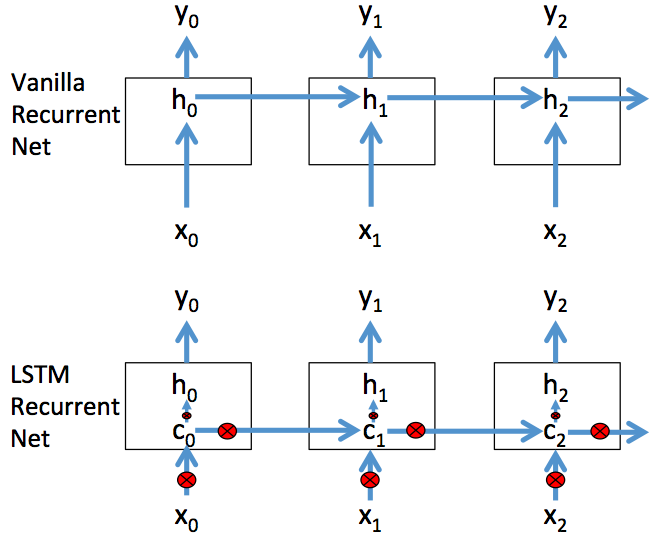
\includegraphics[scale=0.28]{figs/lstm_simpleschematic}}
\blfootnote{*Nice explanation of LSTM and variants here: \url{http://colah.github.io/posts/2015-08-Understanding-LSTMs/}}
\end{frame}

%%% 
\begin{frame}
\frametitle{LSTM in detail \cite{gers02peephole}}

\centerline{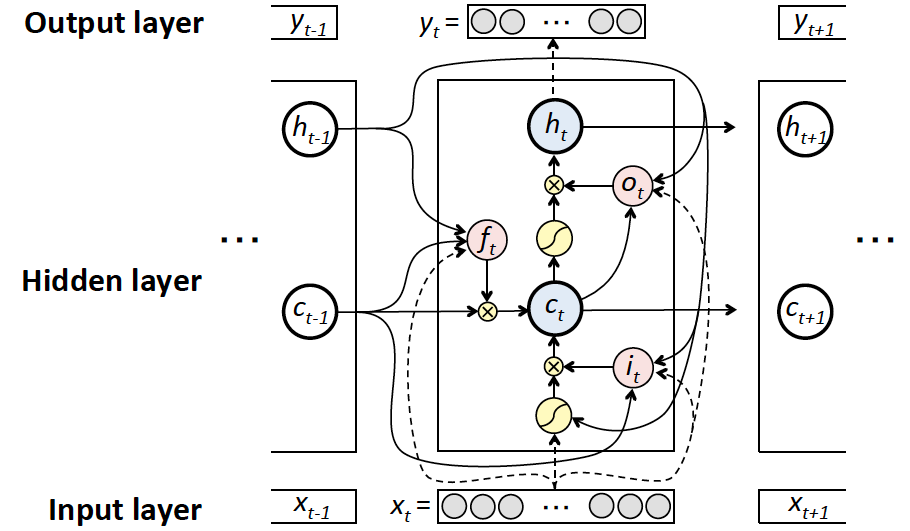
\includegraphics[scale=0.28]{figs/lstm_detailschematic}}
\vspace{-0.4cm}
\begin{eqnarray*}
  i_{t} &=&  \sigma (W_{xi} x_{t} + W_{ci} c_{t-1} + W_{hi} h_{t-1}) \\[-.25em]
  f_{t} &=&  \sigma (W_{xf} x_{t} + W_{cf} c_{t-1} + W_{hf} h_{t-1}) \\[-.25em]
  c_{t} &=&  f_{t} c_{t-1} + \!i_{t} \ tanh (W_{xc} x_{t} + W_{hc} h_{t-1}) \\[-.25em]
  o_{t} &=&  \sigma (W_{xo} x_{t} + W_{co} c_{t} + W_{ho} h_{t-1}) \\[-.25em]
  h_{t} &=&  o_{t} \tanh(c_{t}), \hspace{0.3cm}  y_{t} =  softmax(W_{hy} h_{t})
\end{eqnarray*}
\vspace{-0.2cm}
\blfootnote{Figure courtesy of Adhi Kuncoro \& Yuichiro Sawai}

\end{frame}




%%%%%%%%%
\subsection[Convolution]{Convolution} 

\begin{frame}
\frametitle{Convolution} % frame1
\begin{tikzpicture}[->,>=stealth',shorten >=1pt,auto,node distance=3cm,
  thick,main node/.style={circle,fill=blue!20,draw,font=\sffamily\Large\bfseries}]

  \node[main node] (x1) at (0,0) {$x_1$};
  \node[main node] (x2) at (2,0) {$x_2$};
  \node[main node] (x3) at (4,0) {$x_3$};
  \node[main node] (x4) at (6,0) {$x_4$};
  \node[main node] (x5) at (8,0) {$x_5$};
  \node[main node] (h1) at (2,2) {$h_1$};
  \node[main node] (h2) at (4,2) {$h_2$};
  \node[main node] (h3) at (6,2) {$h_3$};
  	
     \path[red,every node/.style={font=\sffamily\small}]
    (x1) edge node {} (h1)     ;
     \path[blue,every node/.style={font=\sffamily\small}]
    (x2) edge node {} (h1)     ;
   \path[yellow,every node/.style={font=\sffamily\small}]
    (x3) edge node {} (h1)     ;

\end{tikzpicture}
Sliding window of shared weights: $h_j = \sum_{\tau=0}^{2}w_{\tau}x_{j+\tau}$\\[0.2cm]
\end{frame}

%%%%%%%%%
\begin{frame}
\frametitle{Convolution} %frame2
\begin{tikzpicture}[->,>=stealth',shorten >=1pt,auto,node distance=3cm,
  thick,main node/.style={circle,fill=blue!20,draw,font=\sffamily\Large\bfseries}]

  \node[main node] (x1) at (0,0) {$x_1$};
  \node[main node] (x2) at (2,0) {$x_2$};
  \node[main node] (x3) at (4,0) {$x_3$};
  \node[main node] (x4) at (6,0) {$x_4$};
  \node[main node] (x5) at (8,0) {$x_5$};
  \node[main node] (h1) at (2,2) {$h_1$};
  \node[main node] (h2) at (4,2) {$h_2$};
  \node[main node] (h3) at (6,2) {$h_3$};
  
	
     \path[red,every node/.style={font=\sffamily\small}]
    (x2) edge node {} (h2)     ;
     \path[blue,every node/.style={font=\sffamily\small}]
    (x3) edge node {} (h2)     ;
   \path[yellow,every node/.style={font=\sffamily\small}]
    (x4) edge node {} (h2)     ;

\end{tikzpicture}
Sliding window of shared weights: $h_j = \sum_{\tau=0}^{2}w_{\tau}x_{j+\tau}$\\[0.2cm]
\end{frame}

%%%%%%%%%
\begin{frame}
\frametitle{Convolution} %frame3
\begin{tikzpicture}[->,>=stealth',shorten >=1pt,auto,node distance=3cm,
  thick,main node/.style={circle,fill=blue!20,draw,font=\sffamily\Large\bfseries}]

  \node[main node] (x1) at (0,0) {$x_1$};
  \node[main node] (x2) at (2,0) {$x_2$};
  \node[main node] (x3) at (4,0) {$x_3$};
  \node[main node] (x4) at (6,0) {$x_4$};
  \node[main node] (x5) at (8,0) {$x_5$};
  \node[main node] (h1) at (2,2) {$h_1$};
  \node[main node] (h2) at (4,2) {$h_2$};
  \node[main node] (h3) at (6,2) {$h_3$};
 	
     \path[red,every node/.style={font=\sffamily\small}]
    (x3) edge node {} (h3)     ;
     \path[blue,every node/.style={font=\sffamily\small}]
    (x4) edge node {} (h3)     ;
   \path[yellow,every node/.style={font=\sffamily\small}]
    (x5) edge node {} (h3)     ;

\end{tikzpicture}
Sliding window of shared weights: $h_j = \sum_{\tau=0}^{2}w_{\tau}x_{j+\tau}$\\[0.2cm]
\end{frame}

\begin{frame}
\frametitle{Convolution} % frame4
\begin{tikzpicture}[->,>=stealth',shorten >=1pt,auto,node distance=3cm,
  thick,main node/.style={circle,fill=blue!20,draw,font=\sffamily\Large\bfseries}]

  \node[main node] (x1) at (0,0) {$x_1$};
  \node[main node] (x2) at (2,0) {$x_2$};
  \node[main node] (x3) at (4,0) {$x_3$};
  \node[main node] (x4) at (6,0) {$x_4$};
  \node[main node] (x5) at (8,0) {$x_5$};
  \node[main node] (h1) at (2,2) {$h_1$};
  \node[main node] (h2) at (4,2) {$h_2$};
  \node[main node] (h3) at (6,2) {$h_3$};
  	
     \path[red,every node/.style={font=\sffamily\small}]
       (x1) edge node {} (h1)     
        (x2) edge node {} (h2)     
        (x3) edge node {} (h3)     ;

     \path[blue,every node/.style={font=\sffamily\small}]
       (x2) edge node {} (h1)     
        (x3) edge node {} (h2)     
        (x4) edge node {} (h3)     ;

   \path[yellow,every node/.style={font=\sffamily\small}]
      (x3) edge node {} (h1)     
       (x4) edge node {} (h2)     
       (x5) edge node {} (h3)     ;
\end{tikzpicture}
Sliding window of shared weights: $h_j = \sum_{\tau=0}^{2}w_{\tau}x_{j+\tau}$\\[0.2cm]
\end{frame}

\begin{frame}
\frametitle{Pooling} 
\begin{tikzpicture}[->,>=stealth',shorten >=1pt,auto,node distance=3cm,
  thick,main node/.style={circle,fill=blue!20,draw,font=\sffamily\Large\bfseries}]

  \node[main node] (x1) at (0,0) {$x_1$};
  \node[main node] (x2) at (2,0) {$x_2$};
  \node[main node] (x3) at (4,0) {$x_3$};
  \node[main node] (x4) at (6,0) {$x_4$};
  \node[main node] (x5) at (8,0) {$x_5$};
  \node[main node] (h1) at (2,2) {$h_1$};
  \node[main node] (h2) at (4,2) {$h_2$};
  \node[main node] (h3) at (6,2) {$h_3$};
  \node[main node] (p1) at (3,4) {$p_1$};
  \node[main node] (p2) at (5,4) {$p_2$};
  	
     \path[red,every node/.style={font=\sffamily\small}]
       (x1) edge node {} (h1)     
        (x2) edge node {} (h2)     
        (x3) edge node {} (h3)     ;

     \path[blue,every node/.style={font=\sffamily\small}]
       (x2) edge node {} (h1)     
        (x3) edge node {} (h2)     
        (x4) edge node {} (h3)     ;

   \path[yellow,every node/.style={font=\sffamily\small}]
      (x3) edge node {} (h1)     
       (x4) edge node {} (h2)     
       (x5) edge node {} (h3)     ;
     
     \path[every node/.style={font=\sffamily\small}]
       (h1) edge node {} (p1)     
        (h2) edge node {} (p1)     
        (h2) edge node {} (p2)  
        (h3) edge node {} (p2)    ;  
       
\end{tikzpicture}
Max-Pooling nodes: $p_1=max(h_1,h_2)$, $p_2=max(h_2,h_3)$\\[0.2cm]
Advantages of Convolution + Pooling:
\be
\item Fewer weights
\item Shift invariance
\ee
\end{frame}

\begin{frame}
\frametitle{Convolutional Nets in vision \cite{lecun98conv}}
\vspace{0.1cm}
\begin{columns}[c]
    \column{.5\textwidth}
\scalebox{0.55}{\begin{tikzpicture}[->,>=stealth',shorten >=1pt,auto,node distance=3cm,
  thick,main node/.style={circle,fill=blue!20,draw,font=\sffamily\Large\bfseries}]

  \node[main node] (x1) at (0,0) {$x_1$};
  \node[main node] (x2) at (2,0) {$x_2$};
  \node[main node] (x3) at (4,0) {$x_3$};
  \node[main node] (x4) at (6,0) {$x_4$};
  \node[main node] (x5) at (8,0) {$x_5$};
  \node[main node] (h1) at (2,2) {$h_1$};
  \node[main node] (h2) at (4,2) {$h_2$};
  \node[main node] (h3) at (6,2) {$h_3$};
  \node[main node] (h'1) at (3,4) {$p_1$};
  \node[main node] (h'2) at (5,4) {$p_2$};

  \path[every node/.style={font=\sffamily\small}]
    (x1) edge node {} (h1)
    (x2) edge node {} (h1)
    (x3) edge node {} (h1)
    (x2) edge node {} (h2)
    (x3) edge node {} (h2)
    (x4) edge node {} (h2)
    (x3) edge node {} (h3)
    (x4) edge node {} (h3)
    (x5) edge node {} (h3)
    (h1) edge node {} (h'1)
    (h2) edge node {} (h'1)
    (h2) edge node {} (h'2)
    (h3) edge node {} (h'2)
    ;
\end{tikzpicture}}
    \column{.5\textwidth}
{\bf Receptive Field (RF)}: each $h_j$ only connects to small input region via convolution.\\
{\bf Pooling}: e.g. $p_1=max(h_1,h_2)$ or $p_1=\sqrt{h_1^2+h_2^2}$\\[0.2cm]
\end{columns}
\pause
\begin{center}
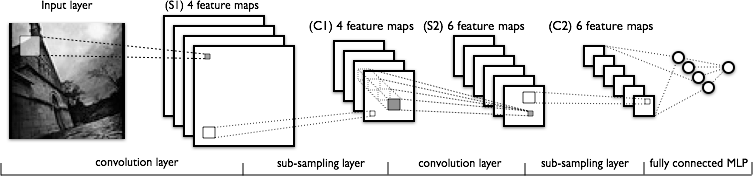
\includegraphics[scale=0.53]{figs/lenet}\\
\tiny{(Figure from \url{http://deeplearning.net/tutorial/lenet.html})}
\end{center}
\end{frame}


%%%%%
\begin{frame}
\frametitle{Section Summary}
\bi
\item RBM
\item Auto-Encoders
\item Recurrent Units
\item Convolution
\ei
\end{frame}
